% !TEX root = ../thesis-example.tex
%
\chapter{Marco de Referencia}
\label{sec:related}

\cleanchapterquote{Si lo que quieres es encontrar los secretos del universo, piensa en términos de energía, frecuencia y vibración}{Nikola Tesla}{(Inventor, ingeniero, físico)}


\section{Metodología}
\label{sec:related:sec1}

Aunque algunas empresas han logrado desarrollar e incluso comercializar rodamientos magnéticos, estos continúan en desarrollo, por lo que no siguen una norma de diseño establecida. Esto implica diseñar una metodología con base en la investigación y desarrollo que han tendido tanto a nivel industrial como académico. Para nuestro caso fueron considerados los siguientes procedimientos: 
\begin{enumerate}
\item Definir a detalle el principio de funcionamiento de los diferentes tipos de rodamientos magnéticos realizando una investigación documental sobre los trabajos e investigaciones que se han hecho al respecto y con esto establecer los requerimientos de diseño.
\item Recopilar información sobre los requerimientos de diseño de los electroimanes y la caracterización de los materiales ferromagnéticos comercializados localmente.
\item Investigación de los tipos de sensores adecuados para las condiciones de operación, seguido por su adquisición o construcción.
\item Plantear un dispositivo de seguridad que sea capaz de sujetar el eje en caso de producirse alguna falla como un corte en el suministro de energía.  
\item Realizar la división por áreas funcionales del proyecto en módulos; definir los diseños conceptuales de cada uno de ellos pensados para la fabricación y validación individual, considerando la futura integración de todos los módulos en una sola estructura. 
\item Realizar los cálculos de la geometría y dimensiones del electroimán, los cuales restringen el tamaño del resto de los componentes. 
\item Realizar el diseño a detalle de los módulos que componen los rodamientos magnéticos activos (radial y axial), módulo de sensores y el módulo de compensación de cargas estáticas.
\item Diseñar la circuitería para la aplicación y control de corrientes en los electroimanes.
\item Diseñar el modulo central para la adquisición de datos y cálculo de fuerzas de corrección. 
\end{enumerate} 


\section{Conceptos Fundamentales}
\subsection{Origen del Campo Magnético}
\label{sec:related:sec2}

Un campo magnético es producido cuando existen cargas eléctricas en movimiento. Estas pueden ser corriente eléctrica (Oersted). También pueden ser producidas por un imán permanente, en este caso no existen corrientes convencionales si no el spin y movimientos orbitales de los electrones sobre los átomos del material (corrientes amperianas). Este campo magnético ejerce fuerza sobre conductores con corriente y materiales magnetizados.\\
\begin{equation}
	 d \overrightarrow{H}=  \frac{Id \overrightarrow{l}\times\hat{r} }{4\pi r^{2}}
\end{equation}
La ley de Biot-Savart nos permite calcular la intensidad del campo magnético H generado por un segmento diferencial del corriente eléctrico. Nótese su magnitud decrece con el cuadrado de la distancia.\\
¿Qué forma tiene estos campos? El campo circula alrededor de un conductor simple en la dirección dada por la regla de la mano derecha:\\\\\\\\

\begin{figure}[htb]
\begin{center}
\centering
	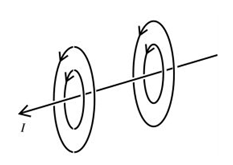
\includegraphics[width=6cm, height=4cm]{images/Capitulo_1/Campo_magnetico_en_un_conductor_sencillo}
	\caption{\textit{Campo magnético en un conductor sencillo.}}
	\label{fig:system:example1}	
\end{center}
\end{figure}
%\vspace*{3cm}
En el mismo año y de manera independiente Ampere dedujo que las cargas en movimiento eran las causas del campo magnético después de enterarse de los experimentos de Oersted. De acuerdo con la ley de ampere el campo magnético generado por un circuito eléctrico depende de la forma del circuito (trayectoria de conducción) y la corriente conllevada. Asumiendo que cada circuito esta echo de un número finito de elementos de corriente, cada uno contribuyendo al campo, integrando estas contribuciones en un punto para determinar el campo ampere concluyo que\\
\begin{equation}
	 \oint {\overrightarrow{H} \cdot d \overrightarrow{l}} =  I_{enc}
\end{equation}

\subsection{Inducción Magnética}
Cuando un campo magnético  H es generado por una corriente, de acuerdo a la ley de ampere,  la respuesta del medio es la inducción magnética B, también llamada densidad de flujo. Todos los medios responden con alguna inducción, en el vacío la relación entre el campo magnetizante y la inducción es \\ 	
						%inserte 3 formula%
Donde  $\mu$0 es la permeabilidad magnética del vacío, un constante universal cuyo valor es de $4\pi\times10^{-7}$

\subsection{Flujo Magnético}

¿Cómo podemos demostrar la presencia de un campo magnético?
Siempre que un campo magnético está presente, existirá un flujo magnético $ \phi$, este flujo y su razón de cambio pueden ser medidos ya que genera una fuerza electromotriz (f.e.m.) en un circuito conductor a través del cual pasa este flujo. Pequeñas partículas como el hierro se alinean con la dirección del flujo. La cantidad de flujo producido depende de las propiedades del medio y varía de un medio a otro.
\begin{equation}
	\phi = \int_{s}^{} \overrightarrow{H} \cdot d \overrightarrow{s}
\end{equation}

El weber es la cantidad de flujo que al ser reducido uniformemente a cero en un segundo produce una f.e.m. de un volt a través de una vuelta de conductor en la que atraviesa tal flujo.
\begin{figure}[htb]
\begin{center}
\centering
	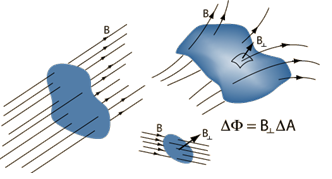
\includegraphics[width=6cm, height=4cm]{images/Capitulo_1/Flujo_magnetico}
	\caption{\textit{Flujo magnetico}}
	\label{fig:system:example1}	
\end{center}
\end{figure}

\section{Materiales Magnéticos}
\label{sec:related:sec3}
\subsection{Magnetización}

En muchos medios $B$ es una función lineal de $H$, en particular se puede decir que $B=\mu_0 H$, Si el valor de $B$ en el vacío es conocido entonces H puede ser inmediatamente calculado.
Sin embargo en otros medio, particularmente materiales ferromagnéticos, $B$ no es una fusión lineal d $H$, ni posee un mismo valor de $H$ para uno de $B$.
Ahora consideramos los efectos que un material tiene sobre la inducción magnética $B$ cuando un campo magnetizaste pasa a través de él. Esto está representado por la magnetización, ente pude ser incrementado en los ferromagnético, o ser reducido como en caso de los diamagnéticos. La permeabilidad relativa del material indica cómo cambia la inducción en el material comparada con la inducción en el vacío.\\\\\\

\begin{figure}[htb]
\begin{center}
\centering
	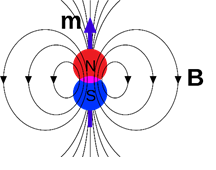
\includegraphics[width=6cm, height=4cm]{images/Capitulo_1/Dipolo_magnetico_de_un_atomo}
	\caption{\textit{Dipolo magnético de  un átomo}}
	\label{fig:system:example1}	
\end{center}
\end{figure}

Para el análisis de materiales magnético es necesario definir cantidades que representen la respuesta de estos materiales ante un campo magnético, estas cantidades son el momento magnético y la magnetización. Una vez que se ha hecho es posible considerar otra propiedad, la susceptibilidad, que está relacionada con la permeabilidad.
Se define una nueva cantidad $M$ (magnetización) como el momento magnético por unidad de volumen
\begin{equation}
	M = \frac{dm}{dV}
\end{equation}

A partir de la relación entre el momento magnético $m$ y el flujo se puede relación $M$ y $B$. Una barra magnética con una densidad $\phi$ en el centro, una longitud de dipolo de l y una área transversal A tiene un momento magnético de $m =\phi \mu_0$  , la magnetización  entonces está dada por $M = \frac{m}{Al}$. Entonces
\begin{equation}
	M = \frac{\phi}{\mu_0A} = \frac{B}{\mu 0}
\end{equation}

En este caso ninguna corriente externa está presente para un campo magnetizante por $B = \mu_0 M$. Podemos ver que la magnetización $M$ y el campo magnetizante $H$ contribuyen a la densidad de flujo en maneras similares.  Ambos magnetización y campo magnético están presentes  entonces sus contribuciones pueden ser sumandos.

\begin{figure}[htb]
\begin{center}
\centering
	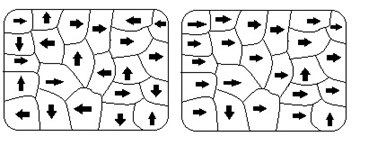
\includegraphics[width=10cm, height=4cm]{images/Capitulo_1/Dominios_magneticos_de_un_material}
	\caption{\textit{Dominios magnéticos de un material no magnetizado (izquierda) y uno magnetizado (derecha)}}
	\label{fig:system:example1}	
\end{center}
\end{figure}

\subsection{Permeabilidad y Susceptibilidad Magnética}

Los diferentes tipos de materiales magnéticos son clasificados de acuerdo a su susceptibilidad y permeabilidad. Entonces debemos de definir estos propiedades antes de describir diferencias entre materiales ferromagnéticos, paramagnéticos y diamagnéticos.
Para materiales isótropos y homogéneos la permeabilidad está definida como:
\begin{equation}
	\mu = \frac{B}{H}
\end{equation}

La susceptibilidad como:

\begin{equation}
	X=\frac{M}{H}
\end{equation}

Dado que $B$ y $M$ pueden o no ser una función lineal de $H$, dependiendo del tipo de material o medio debe de recalcarse que la permeabilidad y susceptibilidad podrían no ser constantes.\\
Es común usar el término permeabilidad relativa $\ mu_r$ definido como:
\begin{equation}
	\mu_r = \frac{\mu }{\mu_0}
\end{equation}

La permeabilidad relativa está relacionada con la susceptibilidad y la siguiente relación siempre es válida:
\begin{equation}
	\mu_r= X+1
\end{equation}

Y su relación con la inducción magnética de la forma:

\begin{equation}
	B=\mu_0 (H + M)
\end{equation}

Los diferentes materiales magnéticos son clasificados de acuerdo a su susceptibilidad. El primer grupo son los materiales  en los que $X$ es pequeña y negativa. Estos materiales son llamados diamagnéticos, su respuesta magnética se opone al campo magnético aplicado. Ejemplos de estos materiales son el cobre, plata, oro.  La superconductores forma otros grupo de diamagnéticos para los cuales $X=-1$.\\
Un segundo grupo de materiales en los que $X$ es pequeña y positiva son los materiales paramagnéticos. La magnetización de los materiales paramagnéticos es débil y alineada con la dirección del campo magnetizante, ejemplos de materiales paramagnéticos son el aluminio, platino y manganeso.\\
A temperatura constante y valores de campo $H$ relativamente bajas la susceptibilidad de los materiales diamagnéticos y paramagnéticos son contantes.

\begin{figure}[htb]
\begin{center}
\centering
	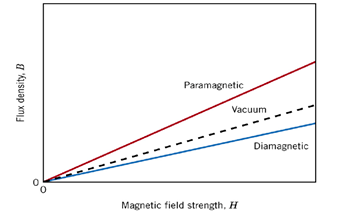
\includegraphics[width=11cm, height=7cm]{images/Capitulo_1/Curva_de_magnetizacion}
	\caption{\textit{Curva de magnetización para materiales paramagnéticos y diamagnéticos con respecto al vacío}}
	\label{fig:system:example1}	
\end{center}
\end{figure}

Los materiales magnéticos más prominentes son los ferromagnetismo, cuya susceptibilidad es positiva y mucho mayor a 1, con valores típicos de $X$ entre los 50 a 10000. Ejemplos de estos materiales son el hierro, cobalto níquel, metales de tierras raras y sus aleaciones.

\subsection{Saturación}
¿Existe un límite para magnetización de un material?
Si un material tiene n dipolos atómicos por unidad de volumen una vez que todos estos dipolos quedan alineados en paralelo se alcanza la magnetización de saturación $M_0$. Se puede realizar una distinción entre la saturación técnica $M_s$  y la saturación Completa $M_0$. 

\begin{figure}[htb]
\begin{center}
\centering
	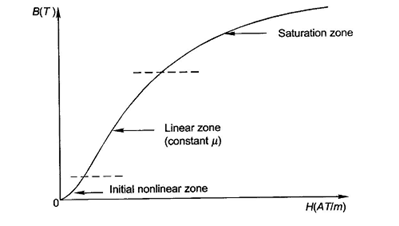
\includegraphics[width=11cm, height=7cm]{images/Capitulo_1/Curva_de_magnetizacion_de_un_material_ferromagnetico}
	\caption{\textit{Curva de magnetización de un material ferromagnético.}}
	\label{fig:system:example1}	
\end{center}
\end{figure}

\subsection{Histéresis}

\begin{figure}[htb]
\begin{center}
\centering
	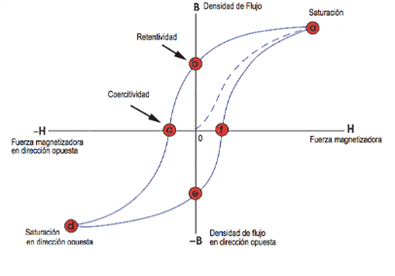
\includegraphics[width=11cm, height=7cm]{images/Capitulo_1/Curva_de_histeresis}
	\caption{\textit{Curva de histéresis.}}
	\label{fig:system:example1}	
\end{center}
\end{figure}

Los efectos de histéresis añaden más complicaciones debido a que la magnetización M  del material depende no solo del campo magnético H como del historial de magnetización del material. Incluso en los casos donde la histéresis ocurre métodos han sido creados para los cálculos de los campos magnéticos en estos dispositivos, en donde la histéresis se tiene en cuenta.

\subsection{Remanecía}

¿Qué le sucede a la inducción magnética de un material ferromagnético una vez que fuerza magnetizante es retirada?\\
Una vez que campo magnetizante es reducido a cero después de magnetizar un material ferromagnético permanece un porción residual de magnetización y por consiguiente una inducción residual donde
\begin{equation}
	B_R=\mu_0 M_R
\end{equation}

En una convención emergente se hace una distinción entre remante y remanencia, donde la remanencia es usada para describir el valor residual de la magnetización después haber llevado el material a saturación, mientras que la magnetización remanente  se refiere al valor residual después de magnetizar el material en un nivel arbitrario.

\subsection{Coercitividad}

La inducción magnética puede ser reducida a cero después de aplicar un campo magnetizante inverso de magnitud $H_c$. Esta intensidad de campo es conocida como coercitividad. Es fuertemente dependiente de la condición de la muestra, siendo afectada por factores como tratamientos térmicos y deformaciones.\\
La coercitividad intrínseca está definida como la intensidad de campo para la cual la magnetización es reducida a cero, en materiales ferromagnéticos suaves $H_c$ y $H_{ci}$ tiene un valor cercano, mientras que en materiales duros está clara una diferencia entre ellas con $H_{ci}$ siendo siempre mayor que $H_c$.

\subsection{Temperatura de Curie}

¿Qué sucede cuando un material ferromagnético es calentado?
Cuando los materiales ferromagnéticos son calentados a temperaturas lo suficientemente altas se convierten en materiales paramagnéticos. La temperatura de transición entre ferromagnetismo y paramagnetismo es ferromagnetismo es conocida como temperatura de Curie. A esta temperatura la permeabilidad de material baja súbitamente y ambas coercitividad y remanencia se vuelven cero.

\subsection{Materiales Ferromagnéticos}

Podemos clasificar los materiales ferromagnéticos en base a su coercitividad. La coercitividad es un propiedad magnética dependiente de la estructura,  esto significa que se puede altera sometiendo al espécimen a diferentes tratamientos térmicos y mecánicos.\\
Fue descubierto que los materiales de a base de hierro con alta dureza mecánica también presentaban una alta coercitividad, mientras que aquellos materiales más maleables tenían una coercitividad menor. Por lo tanto los términos suaves y duros fueron usados para distinguir los materiales ferromagnéticos de acuerdo a esta propiedad. Los materiales duros poseen  una coercitividad sobre los $10K \frac{A}{M}$ mientras aquellos con una coercitividad menor a  $1k \frac{A}{m}$ son considerados suaves.\\
La selección de un material ferromagnético será determinada por las características mostradas en sus lazos de histéresis. Materiales para transformadores necesitan una alta permeabilidad y baja histéresis debido a la necesidad de una alta eficiencia en la conversión de energía eléctrica. Los electroimanes requieren una baja coercitividad y remanencia para reducir fácilmente la magnetización a cero durante el apagado. Finalmente los imanes permanentes requieren de una alta remanencia y coercitividad para retener la mayor magnetización posible. 

\subsection{Aplicaciones de los Materiales Ferromagnéticos}

Electroimánes\\
¿Dónde se usan los materiales ferromagnéticos?
Los materiales ferromagnéticos suaves son usados en electroimánes, motores, transformadores, y relés. Materiales usados en el núcleo de los electroimánes deben de tener una alta permeabilidad, permitiendo alcanzar una lata inducción magnética, al mismo tiempo debe poseer una baja coercitividad de manera que la inducción magnética pueda ser fácilmente revertida.\\
Imanes permanentes\\
¿Dónde usamos materiales ferromagnéticos que quedan permanentemente magnetizado?
Los imanes permanentes son una de las clases más importantes de materiales magnéticos, otros siendo los aceros eléctricos y los imanes de grabación. Los imanes permanentes tienen aplicación in motores eléctricos y generadores, parlantes, televisiones, galvanómetros, dispositivos de suspensión magnética.\\
Para estas aplicaciones el material se  determina a partir de sus histéresis, como la coercitividad y remanencia, es importante resaltar que estas propiedades magnéticas dependen fuertemente de los tratamientos a los que fue sometido el material.\\
En años recientes materiales para imanes permanentes basados en neodimio-hierro-boro han sido descubiertos,  por ejemplo su coercitividad puede ser tan alta como $1.12x106 A/$, comparada con $0.72\times 106$ para samario-cobalto.\\
Además de la coercitividad otro parámetro de vital importancia es el producto energético $BH_{max}$, este es obtenido mediante el producto máximo $BH$ en el segundo cuadrante  de la curva de histéresis,  Este representa la energía magnética almacenada en el material y es usualmente especificado por los fabricantes de imanes permanentes.

\section{Análisis de Circuitos Magnéticos}
\label{sec:related:sec3}

Situaciones en las que la trayectoria del flujo magnético esta interrumpida por un espacio libre (entrehierro) son de gran importancia para las aplicaciones ingenieriles de imanes permanentes, motores, generadores y demás maquinarias eléctricas. \\
Los problemas encontrados aquí son más complicados que  calcular el flujo en un solo material, sin embargo algunas simplificaciones a las ecuaciones de flujo magnético y campo magnetizante pueden usarse para encontrar soluciones a estos problemas.\\
Realizando simplificaciones a partir de las ecuaciones de maxwell, comenzando por la ley de gauss magnética, donde se establece la conservación del flujo magnético alrededor de un nodo.\\
\begin{equation}
	 \oint {\overrightarrow{B} \cdot d \overrightarrow{s}} = 0 \Rightarrow \phi_1 +\phi_2 ... + \phi_i = 0
\end{equation}

La fuerza magnetomotriz $\eta$ como la excitación magnética
\begin{equation}
	Ni = \oint {\overrightarrow{H} \cdot d \overrightarrow{l} = \eta}
\end{equation}

La reluctancia magnética $R$ dependiente de la geometría y material de la muestra
\begin{equation}
	R = \frac{l}{\mu A}
\end{equation}

Y finalmente la relación entre estas, también conocida como ley de Hopkinso

\begin{equation}
	\phi = \frac{\eta}{R}
\end{equation}

\begin{figure}[htb]
\begin{center}
\centering
	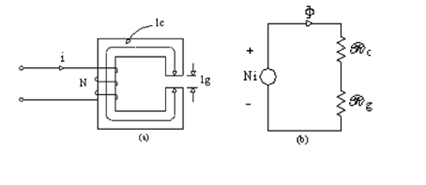
\includegraphics[width=11cm, height=7cm]{images/Capitulo_1/Elementos_de_un_circuito_magnetico}
	\caption{\textit{Elementos de un circuito magnético.}}
	\label{fig:system:example1}	
\end{center}
\end{figure}

A partir de estas ecuaciones es posible el sencillo cálculo del flujo a través de  elementos con diferentes longitudes medias, materiales y secciones transversales mediante las técnicas de análisis de circuitos eléctricos mediante las analogías:\\\\

\begin{tabular}{|c|c|c|c|}
\hline 
Circuitos magnéticos &  & Circuitos eléctricos &   \\ 
\hline
$\eta$ & Fuerza magnetomotriz & $\varepsilon$ & Fuerza electromotriz \\ 
\hline 
$\phi$ & Flujo magnético & $I$ & Corriente eléctrica \\ 
\hline 
 $R$ & Reluctancia & $r$& Resistencia eléctrica\\
\hline
\end{tabular} 

\section{Caracterización de Materiales}
\label{sec:related:sec3}

Para el diseño de electroimánes se requiere conocer las características magnéticas del material, como la permeabilidad relativa y el punto de saturación, sin embargo lo materiales ferromagnéticos comercializados localmente carecen de hojas de especificaciones de donde obtener esta información por lo es necesario disponer de un método para caracterizar sus propiedades más relevantes.

\subsection{Análisis}

A partir de la ley de Faraday que relaciona la variación temporal del flujo eléctrico y la fuerza electromotriz inducida
\begin{equation}
	\varepsilon =\frac{d \lambda}{dt} = \frac{N d \phi}{dt}
\end{equation}

La ley de ampere:
\begin{equation}
	\oint {\overrightarrow{H} d \overrightarrow{l}} = HL = NI \Rightarrow H = \frac{NI}{L}
\end{equation}

Y el concepto de permeabilidad diferencial [cita a la definición de permeabilidad diferencial:
\begin{equation}
	\mu_d = \frac{dH}{dt}
\end{equation}

Es posible obtener una relación entre variables eléctricas medibles (corriente y voltaje)  y la permeabilidad relativa de un núcleo cerrado de longitud promedio L, sección transversal A y N espiras en su embobinado:

\begin{equation}
	\frac{d \phi}{dt} = \frac{d \phi dB}{dB dt} = A \frac{dB}{dt}
\end{equation}
\begin{equation}
	\frac{dB}{dt} = \frac{dB dH}{dH dt} = \mu_d \frac{dH}{dt}
\end{equation}
\begin{equation}
	\frac{dH}{dt} = \frac{dH dI}{dH dt} = \frac{N dI}{L dt}
\end{equation}
\begin{equation}
	\varepsilon = \mu_d (\frac{N^2 A}{l} \frac{dI}{dt})
\end{equation}
\begin{equation}
	\mu_d= \frac{\frac{\varepsilon}{dI}}{dt} (\frac{L}{N^2 A})
\end{equation}

Mediante las mediciones de corriente y voltaje en la bobina se calcula la permeabilidad diferencial para cada punto de I y lo tanto para cada punto de $H$, después de la  integrar la función obtenida $\mu_d (H)$  se puede obtener un aproximado de $B$:
\begin{equation}
	B = \int dB = \int \mu_d dH
\end{equation}

\section{Electroimánes}
\label{sec:related:sec3}
\subsection{Análisis del Electroimán}	

Mediante el análisis de circuitos magnéticos se puede calcular la energía almacenada en el circuito formado por el electroimán.
\begin{figure}[htb]
\begin{center}
\centering
	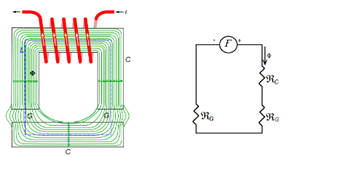
\includegraphics[width=11cm, height=7cm]{images/Capitulo_1/Circuito_magnetico_del_electroiman}
	\caption{\textit{Circuito magnético del electroimán.}}
	\label{fig:system:example1}	
\end{center}
\end{figure}

\begin{equation}
	W_m = \frac{1}{2} Li^2 = \frac{\mu_0 N^2 I^2 A}{2 (\frac{l_e}{\mu_{re}}+ \frac{l_a}{k \mu_{ra}}+ 2y)^2}
\end{equation}

Aplicando el principio de trabajo virtual podemos calcular la fuerza como le variación de la energía con respecto al despeamiento.
\begin{equation}
	F_m = \frac{dW_m}{dy} = - \frac{\mu_0 N^2 I^2 A}{(\frac{l_e}{\mu_{re}}+ \frac{l_a}{k \mu_{ra}}+ 2y)^2}
\end{equation}

Suponiendo que flujo es uniforme sobre la sección transversal núcleo es posible calcular la inducción magnética del material

\begin{equation}
	B = \frac{\phi}{A} = \frac{\mu_0 NI}{\frac{l_e}{\mu_{re}}+\frac{l_a}{k \mu_{ra}+2y}}
\end{equation}

Estas ecuaciones resultan difíciles de trabajar para el diseño del electroimán, sin embargo en el caso de que la condición
\begin{equation}
	u_{r,}y \bracevert 2y >>\frac{l_e}{\mu_{re}} + \frac{l_a}{k \mu_{ra}}
\end{equation}

Sea válida, Los términos que dependen de las longitudes del conductor magnético se vuelven despreciables y las ecuaciones se simplifican a
\begin{equation}
	F_m = - \frac{\mu_0 N^2 I^2 A}{4y^2}
\end{equation}
\begin{equation}
	B = \frac{\mu_0 N I}{2y}
\end{equation}
Gracias a la alta permeabilidad de la ferrita y las condiciones de operación $y_min$   y  $y_max$ estas ecuaciones pueden ser usadas para el cálculo del electroimán.

\section{Imán Permanente}
\label{sec:related:sec3}
\subsection{Análisis del Imán Permanente}

Proponiendo un imán permanente y guía de flujo magnético con la siguiente geometría:
\begin{figure}[htb]
\begin{center}
\centering
	
	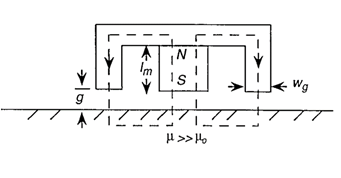
\includegraphics[width=5cm, height=5cm]{images/Capitulo_1/Circuito_magnetico_de_iman_permanente}
	\caption{\textit{Circuito Magnético de imán permanente.}}
	\label{fig:system:example1}	
\end{center}
\end{figure}

\begin{figure}[htb]
\begin{center}
\centering
	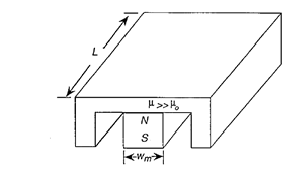
\includegraphics[width=5cm, height=5cm]{images/Capitulo_1/Geometria_de_iman_y_ferrita_guia}
	\caption{\textit{Geometria de imán y ferrita guia.}}
	\label{fig:system:example1}	
\end{center}
\end{figure}

Asumiendo que el plato tiene una permeabilidad relativa infinita y que el imán posee una curva de demagnetización lineal de la forma:
\begin{equation}
	B_m = B_r + \mu_rH_m
\end{equation}

Teniendo en cuenta la falta de fuerza magnetomotriz:

\begin{equation}
	H_m l_m +2Hg = 0 
\end{equation}

Y finalmente la conservación de flujo magnético:
\begin{equation}
	B_m A_m = 2B_g A_g
\end{equation}

Podemos calcular la inducción magnética en el entrehierro:

\begin{equation}
	  B_g(g) = (\frac{A_m}{A_g}) \frac{B_r}{2(1+(\frac{\mu_m}{\mu_0})(\frac{A_m}{A_g})(\frac{g}{l_m}))} 
\end{equation}

Y por consiguiente la fuerza aplicada por el imán permanente debido a una variación en la energía aplicada en el entrehierro.
\begin{equation}
	F_g(g)= \frac{1}{2} \mu_0  \oint \oint B_g^2 ds \hat{n}
\end{equation}
\begin{equation}
	F_g(g)= \frac{1}{2 \mu_0} (2B-^2(g)A_g +B_m^2A_m)  \hat(n)
\end{equation}
\begin{equation}
	F_g(g) = \frac{B_r^2}{2 \mu_0 (1 + (\frac{\mu_m}{\mu_0})(\frac{A_m}{A_g})(\frac{g}{l_m}))^2}[\frac{A_m + 2A_g}{2Ag}] \hat{n}
\end{equation}

Donde
\begin{enumerate}
	\item $A_m$: Es la sección transversal del imán permanente
	\item $A_g$: La sección transversal del entrehierro
	\item $l_m$: La longitud media del imán permanente
	\item $B_r$: La inducción remanente
	\item $H_c$: La coercitividad
	\item $\mu_m$: La permeabilidad magnética del imán permanente definida como  $\frac{B_r}{H_c}$
	\item:$g$ La distancia de entrehierro

\end{enumerate}

\section{Sensores de Desplazamiento}
\label{sec:related:sec3}
\subsection{Requerimientos del Sensor}

Las condiciones de operación del sensor presentan dificultades incluyendo:
\begin{enumerate}
	\item Un rango de operación reducido (1mm a 3mm)
	\item Medición sin contacto 
	\item Inmunidad al ruido de acoplamiento magnético causado por los electroimanes
	\item Rápida respuesta
	\item Resolución mínima  100$um$

\end{enumerate}

\subsection{Tipos de Sensores}
La mayoría de los sensores de desplazamiento de alta precisión requieren de contacto directo como los encoders de cuadratura, potenciómetros y sensores LVDT (Linear Variable Differential Transformer).\\
Los sensores que no requieren de directo con el objeto se basan en la transformación de energía (transductores) o en la medición de alguna propiedad fundamental (resistencia, capacitancia, inductancia) para la detección de esa distancia.\\
Entre los sensores de tipo transductor encontramos los sensores ultrasónicos que:
\begin{enumerate}
	\item Emiten ondas sónicas de alta frecuencia
	\item Las ondas viajan hasta el objeto a detectar y son reflejadas sobre su superficie (siempre y cuando las características del material lo permitan en mayor o menor medida) 
	\item Las ondas reflejadas son detectadas y tiempo entre la transmisión de onda y la recepción es medido. Este tiempo es función directa de la distancia del objeto y la velocidad de propagación en el medio por que la distancia es calculada
\end{enumerate}

Estos sensores tienen la desventaja de poseer un rango mínimo de 10-20$cm$ y un rango máximo determinado por la potencia de la señal transmitida. Estas características. Además del tamaño del transductor no parecen ser una solución al problema de medición.\\
Otros sensores de operación similar son los sensores de tipo “time of fligth” (tiempo de vuelo), estos operan emitiendo un haz de luz no visible en lugar de ondas ultrasónica, poseen un rango reducido, su resolución es baja y su tiempo de respuesta es lento.\\
Los inductivos son especialmente útiles para la detección de materiales metálicos y ferromagnéticos pero debido a la presencia de un campo variable generado los electroimanes adyacentes sus mediciones podrían presentar errores debido a la interferencia.\\

Por otro lado los sensores capacitivos presentan una alta resolución, rango reducido y una detección de objetos no aterrizados y sin contacto siempre y cuando el objeto posea una permitividad mayor a la del vacío, además de poseer una respuesta ultrarrápida.

\subsection{Sensores de Desplazamiento Capacitivo}
A continuación se describen las propiedades básicas de la tecnología de sensores capacitivos y sus aplicaciones industriales. 
Características de los capacitores\\
Los capacitores son el bloque de construcción en el mundo electrónico. Para entender cómo operan estos sensores es importante entender las propiedades y principios fundamentales de los capacitores. Esta sección describe los aspectos físicos, geométricos, y eléctricos de los capacitores.\\
Los capacitores son dispositivos que consisten en dos electrodos separados por un aislante, los capacitores generalmente se componen de dos placas conductivas separadas por un material no conductivo llamado dieléctrico. La energía eléctrica o carga es almacenada en estas placas. \\
Una vez que un voltaje es aplicado a través de las terminales del capacitor los platos conductivos comenzaran a almacenar energía electica hasta que la diferencial de potencial entre estas iguale al voltaje aplicado por la fuente de voltaje.
La carga eléctrica permanece en las palcas incluso después de desconectar la fuente de voltaje a menos que otro componente consuma esta carga o el capacitor se descargue a cusa de las fugas de corriente debido la imperfecciones del aislante dieléctrico.
Sensores de desplazamiento capacitivos\\
Un sensor de capacitivo convierte el cambio eléctrico entre dos conductores en una señal eléctrica. Los sensores se construyen variando algunos de los parámetros que influyen en la capacitancia que según  la ecuación  de capacitancia entre placas paralelas serian el área, la distancia entre placas  o la permitividad del dieléctrico.
$C=F(d,A,\varepsilon_r)$\\
Un sensor de proximidad es un transductor que es capaz de detectar la presencia de un objeto sin contacto físico, normalmente un sensor de proximidad emite alguna campo electromagnético o electrostático, o un haz de radiación electromagnética (radiación infrarroja) y detecta cualquier cambio en el campo o señal de retorno. Sensores de proximidad capacitivo consisten en un oscilador cuya frecuencia está determinada por la capacitancia del circuito al cual los electrodos están conectados, cuando un conductor aterrizado o un material con una alta permeabilidad electica se acercan al electrodo la capacitancia cambia la frecuencia del oscilador. Este cambio es detectado y enviado a la unidad de control. El objeto detectado se le refiere comúnmente como objetivo.
El campo eléctrico distribuido alrededor del capacitor experimenta un cambio el cual es detectado por la unidad de control.

\begin{figure}[htb]
\begin{center}
\centering
	
	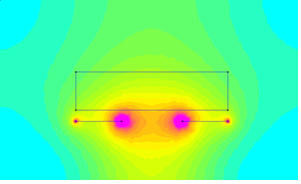
\includegraphics[width=5cm, height=5cm]{images/Capitulo_1/Interaccion_del_campo_electrico_en_un_capacitor_aire}
	\caption{\textit{Interacción del campo eléctrico en un capacitor de placas coplanarias con espacio frontal relleno de aire .}}
	\label{fig:system:example1}	
\end{center}
\end{figure}

\begin{figure}[htb]
\begin{center}
\centering
	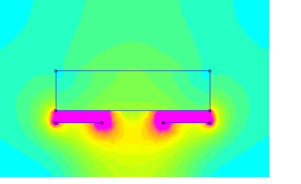
\includegraphics[width=5cm, height=5cm]{images/Capitulo_1/Interaccion_del_campo_electrico_en_un_capacitor_aire_dielectrico}
	\caption{\textit{Interacción del campo eléctrico en un capacitor de placas coplanarias con espacio frontal relleno de dieléctrico.}}
	\label{fig:system:example1}	
\end{center}
\end{figure}

La distancia máxima que el sensor de proximidad es capaz de detectar es conocido como rango nominal. Algunos sensores tienen ajustes del rango nominal o maneras de reportar una detección graduada de la distancia, un sensor de proximidad ajustado a un rango muy limitada es comúnmente referido como un sensor táctil. Los sensores capacitivos usualmente tienen el doble de rango los sensores inductivos.\\



Susceptibilidad a capacitancias parasitas
Los electrodos del sensor poseen capacitancias en el rango de fracción de picofaradios y conectar esas señales a un cable coaxial de 60pF por metro podría obscurecer totalmente la señal. Sin embargo con el blindaje correcto al igual que cualquier otra capacitancia parasita es posible eliminar en mayor medida los efectos  del ruido.
Susceptibilidad al ruido\\
Un peligro para los circuitos osciladores  es que la frecuencia variaría de manera intermitente en el caso de existiría interferencia cruzada causada por circuitos adyacentes, estos problemas pueden ser resueltos mediante un blindaje, una correcta disposición de pistas e integrados en el circuito y el  uso de capacitores de “bypass” en las fuentes de alimentación.\\
Distancia entre los electrodos\\
La capacitancia depende del entrehierro o distancia entre los electrodos conductivos. Esta distancia pude incrementar o decrementar dependiendo de las condiciones ambientales, y del material que podrían generar un mediciones poco exactas, por ejemplo suciedad en la superficie del sensor.



\section{Modelado dinamico, control y simulacion}

Ahora que diseñamos los sensores y actuadores podemos continuar con el modelado dinamico del eje y el control.
A cotinuacion se presenta:
\begin{itemize}
\item El modelo dinamico del rotor
\item La linearizacion del modelo dinamico
\item El diseño de various esquemas de control
\item El algoritmo final de control
\end{itemize}


\subsection{Modelado dinamico}
\subsection{Conceptos de sistemas}
Un sistema es un objeto o proceso en el cual se tiene al menos una entrada y una salida bien definidas. Estos suelen representarse mediante un bloque mostrando sus respectivas entradas y salidas.  

\begin{figure}
\begin{center}
\centering
%\missingfigure[figwidth=6cm]{Diagrama de bloque de un sistema}
\caption{Representacion de bloque de un sistema}
\end{center}
\end{figure}

Un sistema que responde a un entrada con una salida, unicamente pdespues de que esta fue aplicada es conocido como causal.
Lo que se busca en el modelado es, a partir de un conjunto de un 
conjunto de leyes fisicas llegar a un sistema de ecuaciones diferenciales que despues 
seran de ayuda para diseñar un control adecuado. Debido a la naturaleza mixta del 
sistema, las ecuaciones resultantes incluiran terminos tanto del dominio mecanico como 
del dominio electromagnetico. Posteriormente este conjnto de ecuaciones no lineales seran linearizadas con fin de aprovechar las tecnicas de control moderno.


\subsection{Sistemas dinamicos}
Un sistema es cualquier proceso o 

En parte se pueden clasificar como:
\begin{itemize}
\item lineales o no lineales
\item Deterministicos o Estocasticos
\item Variantes o invariantes en el tiempo
\end{itemize}

\subsection[1]{LTI}
Los sistemas lineales invariates en el tiempo (LTI por sus siglas en ingles) son sistemas que tienen una ecuacion diferencial de la forma


%%$$ a_n\frac{d^ny}{dt^n} + a_n-1\frac{d^n-1y}{dt^n-1} 
%%+ a_1\frac{dy}{dt} +a_0y+ = F$$
Este tipo de ecuaciones tienen co
\subsection{Dinamica de una particula}

Ley de Newton
La ley de newton establece que 
$$ \vec{F} = m\vec{a} $$
para una masa puntual con grado de libertad esta equacion puede
escribirse como
$$ \frac{d^2x}{dt^2}=\frac{F(t,x)}{m}$$
la cual es una ecuacion diferencial de segundo grado donde la fuerza puede ser una
funcion dependiente de la posicion $x$ y del tiempo $t$.
Donde $F$ es el conjunto de fuerzas que actuan sobre la particula, si estas fuerzas pueden ser representadas como una combinacion lineal de derivadas de la posicion $x$ de la forma.

\subsection{Dinamica de un cuerpo rigido}

Momento de inercia

Torque y aceleracion angular

Ecuaciones de euler

Precesion
\subsection{Integrando los electroimanes}
\subsection{Linearizacion}
\section{Control}
\subsection{Control retroalimentado}
\subsection{Control integral}
\subsection{Control calendarizado}
\subsection{Discretizacion de controladores}
\subsection{Accionamiento hibrido}

